\chapter{Usage Guide}
\label{chap:usage_guide}

This section is aimed at describing the general use of the software. Such
information is grouped by the different kinds of actors.
Such actors are expected to use the software to perform some
processes or workflows (called here procedures) using the concerned software
\textbf{(including installation procedures)}.

The description of the processes should be organised to facilitate learning by
presenting simpler, more common, or initial processes before more complex, less
utilised, or subsequent processes.

Common procedures should be presented once to avoid redundancy when they are
used in more complex procedures. 

Each process has to be documented using the following use-case textual description
template \cite{armour01usecase} \textbf{BUT its content must be as low level as possible with actual values}:
\vspace{0.5cm}
\hrule
\begin{lyxlist}{UC1}
\small{
\item [\textbf{Use~Case:}] ProcessMissionOne
\item [\textbf{Scope:}] Crisis Management System (\emph{CMS})
\item [\textbf{Primary Actor}:] Coordinator John
\item [\textbf{Secondary Actor}:] FirstAidWorker Bob,\\
                  ExternalResourceSystem (ERS)
\item [\textbf{Intention:}]The intention of the Coordinator is to process mission with ID equal to 1.
\item [\textbf{Level}:]Sub-functional level
\item [\textbf{Main~Success~Scenario}]:\\
1. \emph{John} instructs the \emph{CMS} to process a specific mission.\\
2. \emph{CMS} selects the internal worker \emph{Bob} to execute the mission.\\
3. \emph{CMS} instructs `\emph{Bob} to behave as \emph{FAW}.\\
4. \emph{Bob} informs to the \emph{CMS} of his arrival.\\
5. \emph{Bob} executes the mission.\\
6. \emph{Bob} informs to the \emph{CMS} the mission outcome.


\item [\textbf{Extensions}]:\\
2.a None internal worker can execute the mission.\\
\hspace*{0.5cm} 2.a.1 \emph{CMS} requests an external resource to \emph{ERS}.\\
\hspace*{0.5cm} 2.a.2 \emph{ERS} informs \emph{CMS} that the request can be processed.\\
\hspace*{1.4cm} Use case continues at step 3.

}

\end{lyxlist}
\hrule
\vspace{0.5cm}

\Remark{Graphical User Interfaces (GUIs)}: include GUIs screenshots to show the
different stages of the process while its is performed by the actor.



\section{Actors common procedures}
Common procedures to several actors are grouped in this section to avoid
redundancy.

\subsection{MyCommonProcedure1}

\subsection{MyCommonProcedure2}


\section{Human}

\subsection{ugProcedureAddEvent}
\begin{lyxlist}{UC1}
\small{
\item [\textbf{Use~Case:}] ugProcedureNewEvent
\item [\textbf{Scope:}] Crisis Management System (\emph{CMS})
\item [\textbf{Primary Actor}:] Human Witness Sara
\item [\textbf{Secondary Actor}:] Central Coordinator Tim,\\
                  Communication Company Orange
\item [\textbf{Intention:}]The intention of the Coordinator is to add an new
event to the system.
\item [\textbf{Level}:]User-goal level
\item [\textbf{Main~Success~Scenario}]:\\
1. \emph{Sara} notifies \emph{Orange} that she wants to contact the emergency
central.\\
2. \emph{Orange} puts \emph{Sara} into contact with \emph{Tim} including her
location's information.\\
3. \emph{Tim} confirms \emph{}{Sara}'s situation.\\
4. \emph{Tim} submits the new event to the \emph{CMS}.\\
}
\end{lyxlist}

%\begin{figure}[!ht]
%\centering
%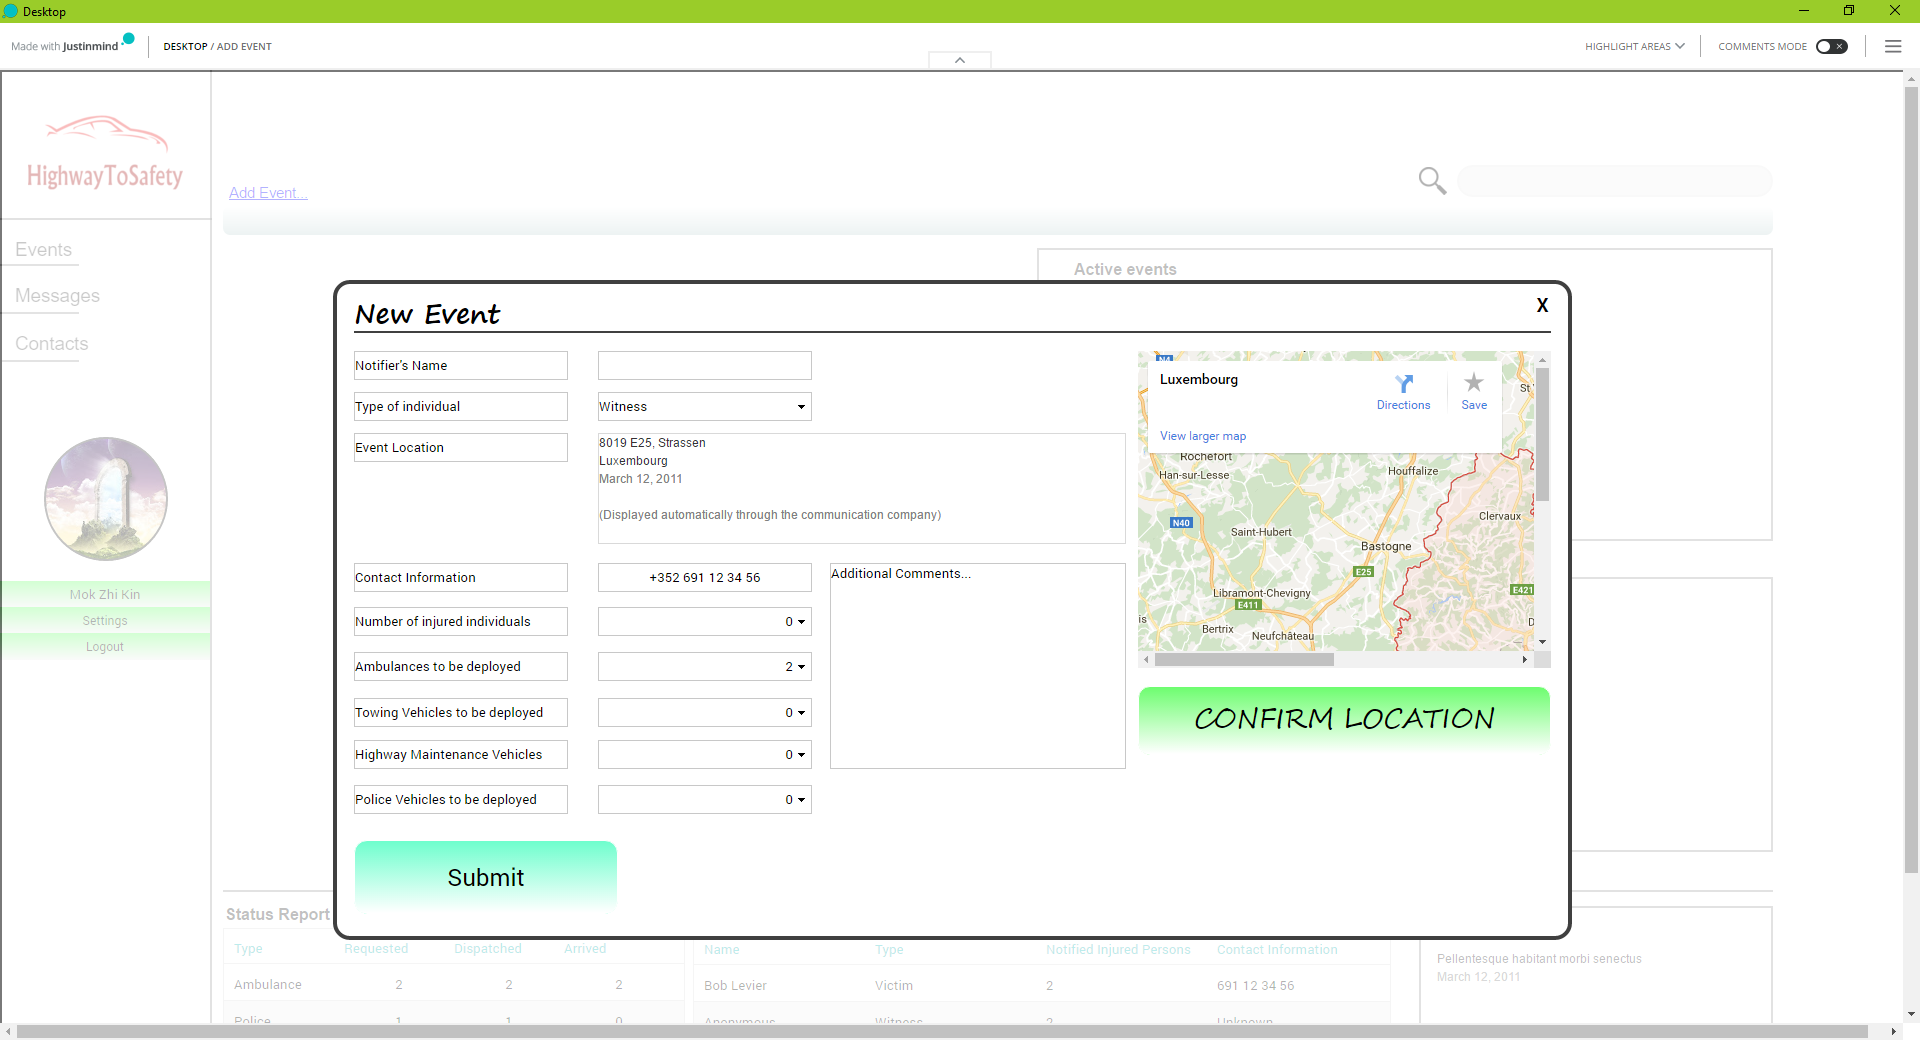
\includegraphics[scale=0.5]{AddNewEventScreenShot.eps_tex}
%\end{figure}



\subsection{MyProcedure2}




\section{My-Actor2 procedures}
\subsection{MyProcedure1}
\subsection{MyProcedure2}


\section{My-Actor3 procedures}

\subsection{MyProcedure1}
\subsection{MyProcedure2}















